\documentclass{article}

% if you need to pass options to natbib, use, e.g.:
%     \PassOptionsToPackage{numbers, compress}{natbib}
% before loading neurips_2021

% ready for submission
\usepackage[preprint]{neurips_2021}

% to compile a preprint version, e.g., for submission to arXiv, add add the
% [preprint] option:
%     \usepackage[preprint]{neurips_2021}

% to compile a camera-ready version, add the [final] option, e.g.:
%     \usepackage[final]{neurips_2021}

% to avoid loading the natbib package, add option nonatbib:
%    \usepackage[nonatbib]{neurips_2021}

\usepackage[utf8]{inputenc} % allow utf-8 input
\usepackage[T1]{fontenc}    % use 8-bit T1 fonts
\usepackage[colorlinks=true]{hyperref}       % hyperlinks
\usepackage{url}            % simple URL typesetting
\usepackage{booktabs}       % professional-quality tables
\usepackage{amsfonts}       % blackboard math symbols
\usepackage{nicefrac}       % compact symbols for 1/2, etc.
\usepackage{microtype}      % microtypography
\usepackage{xcolor}         % colors
\usepackage{graphics}       % include graphics
\graphicspath{ {./fig/} }   % standard path to image folder

\title{Analyzing the Effects of Different Features\\ on Remote Workers' Salaries}

% The \author macro works with any number of authors. There are two commands
% used to separate the names and addresses of multiple authors: \And and \AND.
%
% Using \And between authors leaves it to LaTeX to determine where to break the
% lines. Using \AND forces a line break at that point. So, if LaTeX puts 3 of 4
% authors names on the first line, and the last on the second line, try using
% \AND instead of \And before the third author name.

\author{%
  Tim Weisbarth\\
  Matrikelnummer 5673676 \\
  \texttt{tim.weisbarth@student.uni-tuebingen.de} \\
  \And
  Manuel Arns\\
  Matrikelnummer 6088776\\
  \texttt{manuel.arns@student.uni-tuebingen.de} \\
}

\begin{document}

\maketitle

\begin{abstract}
We are planning to use a dataset containing \href{https://salaries.ai-jobs.net/download/}{remote workers' salaries} to analyze the influence of different features like company size, work experience, job title, company location, company size, and remote ratio on the salaries. We will use regression, analysis of variance, and a choropleth map for this purpose.
\end{abstract}

\section{Introduction}
There are many reasons why workers are paid the way they are. One might have certain assumptions of what factors have the biggest effect on a job's salary; however, these may not hold true. Especially remote desk jobs have many factors that could or could not determine what a worker's labor is worth. The only way to know for sure, is to create some statistical evidence. This report is an attempt to do so using a dataset on remote work salaries.

A data analysis pipeline, comprised of data collection, preprocessing, analysis, and visualization, helps us identify the given features' influence. The following chapters describe these elements in appropriate detail. Furthermore we discuss the analysis results and attempt to put them into context.

%Why this question is interesting:\\
%- more and more people consider to work remotely\\
%- especially during corona times it seems not to matter anymore (I think we should not %get into this, as we are not making a comparisson to non-remote work and therefor this %is pure speculation and has nothing to do with our analysis)\\
%--> But we dont really compare it to non-remote?\\
%- elaboration on question\\

\section{Data Collection}
The data was collected by a project called \href{https://salaries.freshremote.work/download/}{Fresh Remote Work salaries}. The projects' website states: "This site collects salary information anonymously from professionals all over the world in the Remote Work space and makes it publicly available for anyone to use [and] share. The primary goal [of the project] is to have data that can provide better guidance in regards to what's being paid globally. So newbies, experienced pros, hiring managers, recruiters and also startup founders or people wanting to make a career switch can make better informed decisions." Anyone, willing to share his salary information, can fill out a short form on the website consisting of 10 mandatory questions. It is unclear how and whether this user data is preprocessed before being added to the provided dataset. 

Duplicate rows DevOps
--> other datasets not used bc 

%Similar websites \href{https://github.com/foorilla}{More similar datasets}

\section{Data Analysis}
\subsection{Methods}
\subsubsection{Correlation Coefficient}
The most commonly used pearson correlation coefficient can not be applied to the dataset because not all variables are normally distributed. Instead, the Spearman correlation coefficient is used. This coefficient only requires that the correlation between two variables is monotonic and can be ranked which we assume to be the case. For any two variables $x$ and $y$ it is defined as

\begin{equation}
    r_s = \frac{\Sigma(R(x), R(y))}{\sigma(R(x)) \cdot \sigma(R(y))}
\end{equation}

where $\Sigma(x, y)$ denotes the covariance, $R(x)$ the rank, and $\sigma(x)$ the standard deviation. It is the Pearson coefficient between the rank of the two variables \cite{spearman1904proof}.

\subsubsection{Linear Regression}
In this paper ordinary least squares linear regression is used, as it was introduced in the lecture. It is used to analyse the influence of different features on the salaries and implemented using sklearns' LinearRegression class. In order to quantify how well this model predicts the salaries, the coefficient of determination $R^2$ is used. $R^2$ describes the proportion of the variance of the salaries $s_i$ which can be explained through the linear regression estimate $\hat{s_i}$. It is calculated by the standard formula

\begin{equation}
    R^2 = \frac{\sum_{i=1}^{n} (\hat{s_i} - \bar{s})^2}{\sum_{i=1}^n ({s_i} - \bar{s})^2}
\end{equation}

where $\bar{s}$ denotes the mean average salary and $\hat{s_i}$ the fitted value. 

% Does sklearn automatically use some regularization or similar?

\subsubsection{Choropleth Map} % ---> maybe this section should come before lin reg
We consider it intuitive, that the country in which a company is located could have a large impact on their employee's salary. As this information is not numeric, it cannot be analyzed with linear regression. We choose to generate a choropleth map that shows the mean average salary for each country.

\subsection{Data Preprocessing}
The salaries data contains some features that need to be processed in order to fit the requrements of the analysis methods and produce the best possible results. This is done through a preprocessing pipeline. The individual steps of this pipeline are described in the following.

\paragraph{Country Code Extension:}
The location information in the salary data follows the \textit{ISO 3166 Alpha 2} standard for country codes, while the map and GDP data's location information follow the \textit{Alpha 3} standard. In order to merge these dataframes, this processing step converts the \textit{Alpha 2} codes of the salary data to the \textit{Alpha 3} format.

\paragraph{GDP per Capita:}
This step calculates a GDP per capita based on the GDP and population estimates provided by the world dataset. As this figure is generally a good indicator of a countries economical success, we suspect it to also indicate salaries.

\paragraph{Same Country Attribute:}
The salaries data provides both the country of residence of the employees, and the company location. This allows us to see, whether an employee works in the same country as he lives. To see if this might have an impact on salary, we create a feature that encodes this binary information.

\paragraph{Non-Numeric to Numeric:}
The workers experience level, work year, and the companies size in the salaries data are represented by non-numeric data types. As all these are rankable, we choose to represent them using integers, so they can be used for Spearman correlation analysis and linear regression.

\paragraph{AI/ML Attribute:}
We define a new attribute in the salary data, encoding whether an employee is working in an AI or ML type position or not.

\paragraph{Outlier Detection:}
Of the employed methods, linear regression in particular is prone to be strongly influenced by outliers. To combat this we drop the top and bottom 2\% of salary data. We found this value to be a good trade-off between loss of data and imporvement of analysis result.

In addition to this general preprocessing pipeline, all numeric values are normalized before linear regression.

%- Drop Nan\\ ---> IMO not necessary to mention
%    Some countries gdp not provided in geopandas\\

%- Ignore employment type\\ ---> what?
%    low data\\

%- Normalize data\\
%    --> predictors are uncorrelated and normalized\\\\

% Maybe better by country --> world map\\

\subsection{Results}
In this chapter, we discuss the results of the three conducted analyses. Figure \ref{fig:correlations} shows a heatmap containing the Spearman correlation coefficients for all numeric features. Of the highest interest is, of course, the correlation between any feature with the salary in USD.

\begin{figure}[ht]
    \centering
    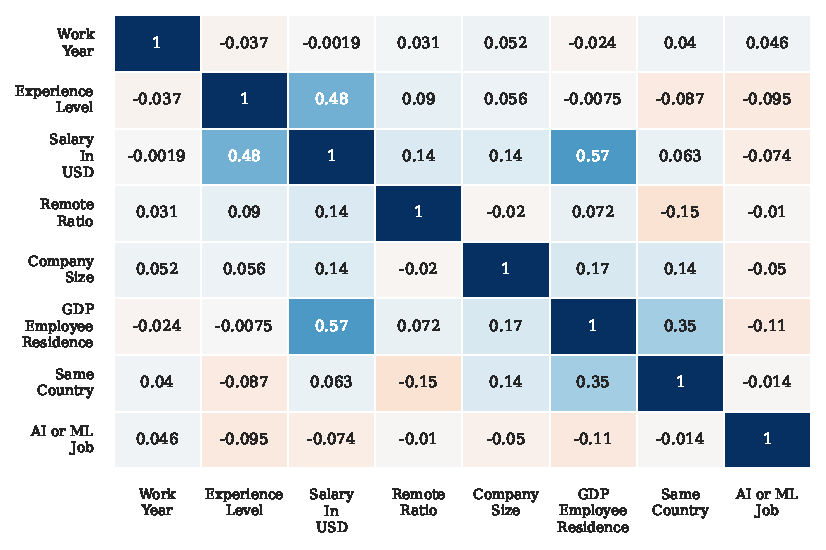
\includegraphics{correlations.pdf}
    \caption{Spearman correlation coefficients for numeric variables.}
    \label{fig:correlations}
\end{figure}
% Question: Drop one GDP value and say we did so because of the high correlation? Or should we keep both in plot

\begin{figure}[ht]
    \centering
    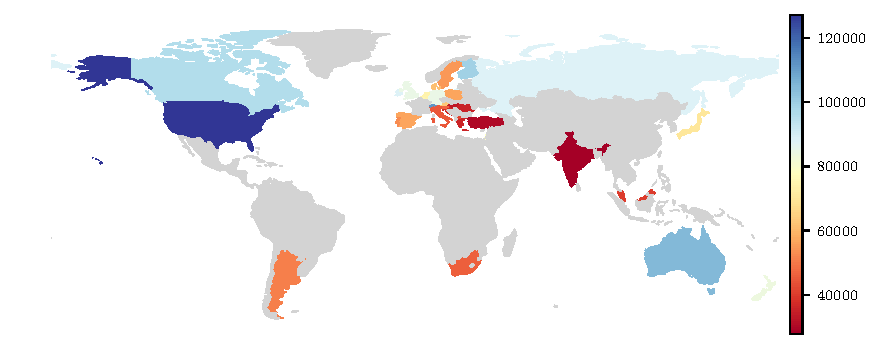
\includegraphics{choropleth.pdf}
    \caption{Multivariate linear regression results for VARIABLE and VARIABLE.}
    \label{fig:regression}
\end{figure}

\subsection{Regression}
The multiple linear regression (MLR) takes as predictors all attributes visible in Figure \ref{fig:correlations}. The highest weight were associated to the attribute GDP Employee residence with $0.56$, Experience Level with $0.46$ and the same country attribute with $-0.11$. The weights of all remaining predictors are smaller or equal to $0.06$. The coefficient of determination of the MLR is $0.52$.\\

Figure ... 

Caption: Regression for attribute gdp\_company\_location and target salray\_in\_usd with all datapoints and means. 

The US


%        --> quadratic approach has not brought\\ improvement (to be tested for some %predictors)
%        --> Biggest group: maybe improvement? Software, data group?\\


\begin{figure}[ht]
    \centering
    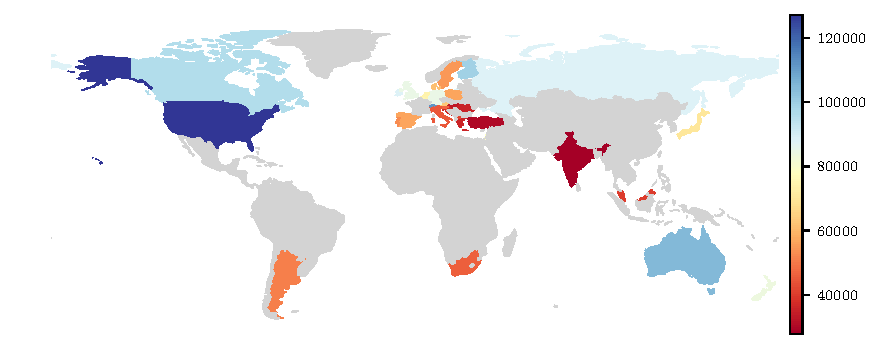
\includegraphics{choropleth.pdf}
    \caption{Choropleth map of mean average salary in USD per country.}
    \label{fig:choropleth}
\end{figure}

%Two main influences were found: Country (represented by country gdp) and Experience %Level

\section{Outlook}
%Alternativen: HDI anstatt Gdp?, gemeinsames Datenset betrachten? Datensatz wächst!, quadratische %anstatt lineare Regression? Job-Gruppenweise Regression?\\

\bibliographystyle{plainnat}
\bibliography{bibliography.bib}

\end{document}
